% !TEX program = xelatex
\documentclass[12pt,a4paper,fontset=fandol]{ctexart}
\usepackage[left=22mm,right=22mm,top=22mm,bottom=22mm]{geometry}
\usepackage{amsmath,amssymb,bm,mathtools}
\usepackage{graphicx,xcolor,booktabs,longtable,array,calc}
\usepackage{tikz}
\usetikzlibrary{arrows.meta,calc,decorations.pathmorphing}
\usepackage{setspace,enumitem,fancyhdr}
\usepackage[unicode,hidelinks]{hyperref}
\setstretch{1.24}
\setlength{\parindent}{2em}
\setlength{\parskip}{.35em}
\setlength{\emergencystretch}{2em}
\setlist{nosep,leftmargin=2em}
\setcounter{secnumdepth}{-1}
\ctexset{section={format=\Large\bfseries,beforeskip=1em,afterskip=.7em},
subsection={format=\large\bfseries,beforeskip=.8em,afterskip=.4em},
subsubsection={format=\normalsize\bfseries,beforeskip=.7em,afterskip=.3em}}
\allowdisplaybreaks[2]
\tikzset{arr/.style={-{Stealth[length=2mm]},semithick},
dot/.style={circle,fill,inner sep=1.5pt}}
\providecommand{\tightlist}{\setlength{\itemsep}{0pt}\setlength{\parskip}{0pt}}
\providecommand{\pandocbounded}[1]{#1}
\newsavebox{\diagrambox}
\pagestyle{fancy}
\fancyhf{}
\renewcommand{\headrulewidth}{0pt}
\fancyfoot[C]{\small \thepage}
\setlength{\headheight}{16pt}
\begin{document}
\begin{titlepage}
\thispagestyle{empty}
\vspace*{27mm}
\begin{center}
{\LARGE\bfseries 第37届全国中学生物理竞赛\par}
\vspace{8mm}
{\LARGE\bfseries 复赛理论试题\par}
\vspace{17mm}
{\Large 试题版\par}
\end{center}
\vfill
\end{titlepage}
\setcounter{page}{1}
本卷共8题，总分320分。考试时间：9:00-12:00。所有需要评阅的解答均须写在答题纸上。

\section{第 1
题　双气室空气弹簧的刚度（40分）}\label{ux7b2c-1-ux9898-ux53ccux6c14ux5ba4ux7a7aux6c14ux5f39ux7c27ux7684ux521aux5ea640ux5206}

高铁空气弹簧由承载主气室和容积不变的附加气室组成，以阀门连通，如图。气囊内的压缩空气对簧上负载提供竖直向上的作用力。负载平衡时，主室压强、体积为\(p_{10},V_{10}\)，附加室容积为\(V_2\)，大气压为\(p_0\)。定义有效承载面积\(A_e=F/(p_1-p_0)\)，其中\(F\)是向上的气囊作用力，\(p_1\)是主室气体压强。

\begin{center}
\begin{minipage}{\linewidth}
\centering\begingroup\sbox{\diagrambox}{\small
\begin{tikzpicture}[scale=.9]
\draw[thick,fill=gray!8] (-.3,3) rectangle(2.7,3.6);
\node at (1.2,3.3) {簧上负载};
\draw[thick] (0,2.7)--(0,.5)--(2.4,.5)--(2.4,2.7);
\draw[very thick] (-.1,2.7)--(2.5,2.7);
\node at (1.2,1.5) {主室$p_1,V_1$};
\draw[thick] (-4,.5) rectangle(-2.2,2.2);
\node at (-3.1,1.4) {附加室$V_2$};
\draw[thick] (-2.2,1)--(-1.5,1)--(-1.5,2.1)--(0,2.1);
\draw[thick] (-1.2,1.9)--(-.8,2.3); \draw[thick] (-1.2,2.3)--(-.8,1.9);
\node[above] at (-1,2.5) {阀门};
\draw[arr] (3,2.7)--(3,1.9) node[below] {$y>0$};
\draw[arr,red] (1.2,3.6)--(1.2,4.5) node[above] {$F=(p_1-p_0)A_e$};
\node at (-.7,-.25) {主室随位移改变；附加室容积固定};
\end{tikzpicture}
}
\ifdim\wd\diagrambox>.88\linewidth
\sbox{\diagrambox}{\resizebox{.88\linewidth}{!}{\usebox{\diagrambox}}}\fi
\ifdim\ht\diagrambox>.20\textheight
\resizebox{!}{.20\textheight}{\usebox{\diagrambox}}
\else\usebox{\diagrambox}\fi
\par\smallskip{\small 图1a　主室与定容附加室\par}\endgroup\end{minipage}\end{center}

空气定容摩尔热容\(C_V=5R/2\)。微振幅下，主室体积\(V_1\)和有效面积\(A_e\)均是承载面相对平衡位置的竖直位移\(y\)的线性函数，取向下为正，变化率分别为\(-\alpha\)及\(\beta\)，\(\alpha,\beta>0\)。

（1）阀门关闭时，求劲度系数\(K\equiv dF/dy\)与\(A_e\)的关系：（i）上下乘客时气体发生等温变化；（ii）列车剧烈颠簸时气体发生绝热变化。

（2）阀门打开、主室连通附加室后，分别求上述两种情况下\(K\)与\(A_e\)的关系。通道容积忽略。

\clearpage

\section{第 2
题　台球击打后的滑动、滚动与摆线（40分）}\label{ux7b2c-2-ux9898-ux53f0ux7403ux51fbux6253ux540eux7684ux6ed1ux52a8ux6edaux52a8ux4e0eux6446ux7ebf40ux5206}

质量\(m\)、半径\(R\)的均质实心母球静置于水平桌面。球与桌面的滑动摩擦系数为\(\mu\)，最大静摩擦力等于滑动摩擦力。球杆在球心所在的竖直平面内保持水平，击打球的上半部，击打线高于球心水平面\(R/2\)。击打时间极短，母球获得大小\(P\)的水平冲量。重力加速度为\(g\)。

\begin{center}
\begin{minipage}{\linewidth}
\centering\begingroup\sbox{\diagrambox}{\small
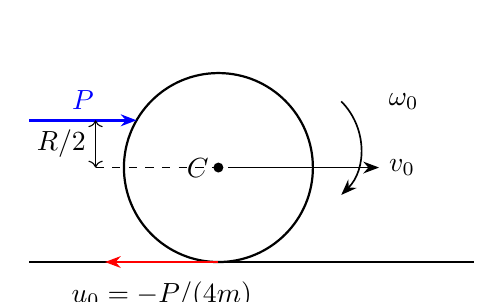
\begin{tikzpicture}[scale=1.2]
\draw[thick] (-2,0)--(2.7,0);
\draw[thick] (0,1) circle(1);
\fill (0,1) circle(1.5pt) node[left] {$C$};
\draw[arr,blue,very thick] (-2,1.5)--(-.866,1.5) node[midway,above] {$P$};
\draw[dashed] (-1.3,1)--(1,1);
\draw[<->] (-1.3,1)--(-1.3,1.5) node[midway,left] {$R/2$};
\draw[arr] (.2,1)--(1.7,1) node[right] {$v_0$};
\draw[arr] (1.3,1.7) arc(45:-45:.7);
\node[right] at (1.7,1.7) {$\omega_0$};
\draw[arr,red] (0,0)--(-1.2,0);
\node[below] at (-.6,-.1) {$u_0=-P/(4m)$};
\end{tikzpicture}
}
\ifdim\wd\diagrambox>.88\linewidth
\sbox{\diagrambox}{\resizebox{.88\linewidth}{!}{\usebox{\diagrambox}}}\fi
\ifdim\ht\diagrambox>.20\textheight
\resizebox{!}{.20\textheight}{\usebox{\diagrambox}}
\else\usebox{\diagrambox}\fi
\par\smallskip{\small 图2a　击打位置与初始接触点运动\par}\endgroup\end{minipage}\end{center}

（1）击打后经过多久母球开始纯滚动？求进入纯滚动时的球心速度。

（2）在开始纯滚动时将计时清零，记此时球上与桌面接触的材料点为\(B\)。求随后\(t'\)时刻\(B\)的位置、速度和加速度。

\clearpage

\section{第 3
题　负微分电阻与RLC振荡（40分）}\label{ux7b2c-3-ux9898-ux8d1fux5faeux5206ux7535ux963bux4e0erlcux632fux836140ux5206}

某些电路或元件在特定电压范围内，电流随端电压增加而减小，称为负微分电阻效应。简化电路如图：左侧由电阻\(R\)、电感\(L\)、电容\(C\)和隧道二极管\(D\)形成交流回路，交流电流为\(i(t)\)；右侧由理想高频扼流圈RFC和理想直流电源\(V_0\)组成，直流电流为\(I\)，\(I\gg|i(t)|\)。RFC直流电阻为零，完全阻断交流。已标示电流方向。

\begin{center}
\begin{minipage}{\linewidth}
\centering\begingroup\sbox{\diagrambox}{\small
\begin{tikzpicture}[scale=.95]
\draw[thick] (0,0)--(0,.6); \draw[thick] (-.2,.6) rectangle(.2,1.4);
\node[left] at (-.2,1) {$R$}; \draw[thick] (0,1.4)--(0,2)--(.5,2);
\draw[thick,decorate,decoration={coil,aspect=.3,segment length=4pt,amplitude=3pt}] (.5,2)--(1.4,2);
\node[above] at (.95,2.25) {$L$};\draw[thick] (1.4,2)--(1.9,2);
\draw[thick] (1.9,1.7)--(1.9,2.3); \draw[thick] (2.1,1.7)--(2.1,2.3);
\node[above] at (2,2.3) {$C$}; \draw[thick] (2.1,2)--(3,2);
\draw[thick] (3,2)--(3,1.4); \draw[thick,fill=gray!12] (2.65,.6) rectangle(3.35,1.4);
\node at (3,1) {$D$};\draw[thick] (3,.6)--(3,0)--(0,0);
\node[right] at (3.4,1) {$r_d=-R_0$};
\draw[thick] (3,2)--(4,2);
\draw[thick,decorate,decoration={coil,aspect=.3,segment length=4pt,amplitude=3pt}] (4,2)--(5,2);
\node[above] at (4.5,2.3) {RFC};
\draw[thick] (5,2)--(6,2)--(6,1.4); \draw[thick] (6,1) circle(.4);
\node at (6,1) {$V_0$};\draw[thick] (6,.6)--(6,0)--(3,0);
\draw[arr,blue] (.7,1.3)--(1.8,1.3) node[midway,below] {$i(t)$};
\draw[arr,red] (5.7,3.1)--(3.4,3.1) node[midway,above] {$I$};
\node at (3,-.7) {左侧交流回路；右侧直流偏置};
\end{tikzpicture}
}
\ifdim\wd\diagrambox>.88\linewidth
\sbox{\diagrambox}{\resizebox{.88\linewidth}{!}{\usebox{\diagrambox}}}\fi
\ifdim\ht\diagrambox>.20\textheight
\resizebox{!}{.20\textheight}{\usebox{\diagrambox}}
\else\usebox{\diagrambox}\fi
\par\smallskip{\small 图3a　直流偏置与交流回路\par}\endgroup\end{minipage}\end{center}

二极管始终处于负微分电阻区，其微分电阻为\(-R_0\)，\(R_0>0\)且为常量。

（1）已知\(i(0)=0\)、\(\dot i(0)=\beta\neq0\)，且

\[
i(t)=\alpha_1e^{\beta_1t}+\alpha_2e^{\beta_2t},
\]

求各常数及任意时刻\(i(t)\)。

（2）求左侧产生持续等幅谐振的条件、电流\(i_H(t)\)和频率\(f_H\)。

（3）求左侧产生随时间衰减的RLC阻尼振荡的条件、电流\(i_D(t)\)及振荡频率\(f_D\)。

（4）二极管负微分电阻工作电压范围为\(V_{\min}\leq V_D\leq V_{\max}\)。求其交流部分能提供的最大平均功率\(\overline P_{\max}\)，以及此时直流电源电压\(V_0\)。

\clearpage

\section{第 4
题　同步加速器磁场与反质子产生阈值（40分）}\label{ux7b2c-4-ux9898-ux540cux6b65ux52a0ux901fux5668ux78c1ux573aux4e0eux53cdux8d28ux5b50ux4ea7ux751fux9608ux503c40ux5206}

回旋加速器利用两个半圆形磁场使带电粒子沿圆弧转向，粒子反复经过两半圆缝隙间的高频电场而获得能量。某同步质子加速器Tevatron的粒子运行最大圆形轨道周长为\(L_{\max}=6436\)
m，可将质子加速到最大能量\(E_{p,\max}=1.00\times10^6\) MeV。

（1）粒子始终在垂直于均匀磁场的平面内运动，不计辐射损失。求达到该最大能量所需要的最小磁感应强度\(B_{\min}\)。

\begin{center}
\begin{minipage}{\linewidth}
\centering\begingroup\sbox{\diagrambox}{\small
\begin{tikzpicture}[scale=1]
\draw[thick] (0,0) circle(2);
\draw[arr] (2,0) arc(0:65:2);
\draw[arr] (0,2)--(-1.4,2) node[left] {$\mathbf p$};
\draw[arr,red] (0,2)--(0,.7) node[left] {$e\mathbf v\times\mathbf B$};
\draw[arr] (0,0)--(2,0) node[midway,below] {$R$};
\foreach \x/\y in {-1/-1,1/1,1/-1}{\node at (\x,\y) {$\otimes$};}
\node at (0,-2.8) {$p=eBR,\quad 2\pi R\leq L_{\max}$};
\node at (3.1,.7) {$\mathbf B$入纸面};
\end{tikzpicture}
}
\ifdim\wd\diagrambox>.88\linewidth
\sbox{\diagrambox}{\resizebox{.88\linewidth}{!}{\usebox{\diagrambox}}}\fi
\ifdim\ht\diagrambox>.20\textheight
\resizebox{!}{.20\textheight}{\usebox{\diagrambox}}
\else\usebox{\diagrambox}\fi
\par\smallskip{\small 图4a　磁场弯转与轨道周长限制\par}\endgroup\end{minipage}\end{center}

（2）高能质子撞击静止质子，可产生反质子，反应为

\[
p+p\longrightarrow p+p+p+\overline p.
\]

求入射质子产生反质子的最小动能，并判断上述加速器能否实现此反应。

已知\(m_pc^2=938.3\) MeV，\(c=3.00\times10^8\)
m/s。第一问给定能量按质子总能量使用。

\clearpage

\section{第 5
题　飞行器间光信号与相对论投递（40分）}\label{ux7b2c-5-ux9898-ux98deux884cux5668ux95f4ux5149ux4fe1ux53f7ux4e0eux76f8ux5bf9ux8bbaux6295ux901240ux5206}

在惯性系\(\Sigma\)的\(Oxy\)坐标中，飞行器甲、乙沿同一条直线朝\(-y\)匀速飞行，丙在与之平行、相距\(d\)的另一条直线上朝\(+y\)匀速飞行。速度为

\[
\mathbf v_{\text{甲}\Sigma}=-\frac{2c}{3}\hat{\mathbf y},
\quad
\mathbf v_{\text{乙}\Sigma}=-\frac c3\hat{\mathbf y},
\quad
\mathbf v_{\text{丙}\Sigma}=\frac{2c}{3}\hat{\mathbf y}.
\]

甲、乙所在直线为\(x=0\)，丙所在直线为\(x=d\)；原图乙在甲的\(-y\)一侧。飞行器尺寸远小于\(d\)。

\begin{center}
\begin{minipage}{\linewidth}
\centering\begingroup\sbox{\diagrambox}{\small
\begin{tikzpicture}[scale=1]
\draw[arr] (-.5,0)--(5,0) node[right] {$x$};
\draw[arr] (0,0)--(0,4.2) node[above] {$y$};
\node[left] at (0,3.4) {甲};\draw[arr,blue] (0,3.4)--(0,2.5);
\node[left] at (0,1.4) {乙};\draw[arr] (0,1.4)--(0,.6);
\draw[dashed] (3.7,0)--(3.7,4);
\node[right] at (3.7,1.4) {丙};\draw[arr,red] (3.7,1.4)--(3.7,2.4);
\draw[<->] (0,-.6)--(3.7,-.6) node[midway,below] {$d$};
\node at (1.8,5.2) {$v_\text{甲}=-2c/3,\ v_\text{乙}=-c/3,\ v_\text{丙}=2c/3$};
\end{tikzpicture}
}
\ifdim\wd\diagrambox>.88\linewidth
\sbox{\diagrambox}{\resizebox{.88\linewidth}{!}{\usebox{\diagrambox}}}\fi
\ifdim\ht\diagrambox>.20\textheight
\resizebox{!}{.20\textheight}{\usebox{\diagrambox}}
\else\usebox{\diagrambox}\fi
\par\smallskip{\small 图5a　三艘飞行器的航线\par}\endgroup\end{minipage}\end{center}

（1）甲向乙发射光信号，乙收到后立即反射回甲。甲上原子钟测得从发射到收到返回光的时间为\(T\)。求\(\Sigma\)中和乙上观察者测得的这两事件的时间间隔；再求在甲系中，从甲收到返回光到甲追上乙的时间。

（2）甲与丙在\(\Sigma\)中相距最近时，甲发射质量和尺寸均可忽略的小货物。货物在\(\Sigma\)中的速率为\(3c/4\)，要求丙恰好收到它。求甲系中货物发射速度的大小及方向，并求乙系中货物从甲发射到丙接收的时间间隔。

\clearpage

\section{第 6
题　光纤导光与旋转环形腔（40分）}\label{ux7b2c-6-ux9898-ux5149ux7ea4ux5bfcux5149ux4e0eux65cbux8f6cux73afux5f62ux815440ux5206}

半径\(R\)的光纤环路以角速度\(\Omega\)旋转，固定在环上的分束器\(A\)分出两束相干光，分别沿逆时针CCW和顺时针CW传播后返回\(A\)。检测两束光的相位差，可以确定转动角速度；真空光速为\(c\)。

\begin{center}
\begin{minipage}{\linewidth}
\centering\begingroup\sbox{\diagrambox}{\small
\begin{tikzpicture}[scale=1]
\draw[thick] (0,0) circle(2);
\fill (0,2) circle(2pt) node[above] {$A$};
\draw[arr,blue,thick] (0,2) arc(90:155:2); \node[blue] at (-2.8,1.2) {CCW};
\draw[arr,red,thick] (0,2) arc(90:25:2); \node[red] at (2.8,1.2) {CW};
\draw[arr] (1,0) arc(0:90:1); \node at (.8,.8) {$\Omega$};
\draw[arr] (0,0)--(2,0) node[midway,below] {$R$};
\node at (0,-2.7) {光传播与移动分束器相遇};
\end{tikzpicture}
}
\ifdim\wd\diagrambox>.88\linewidth
\sbox{\diagrambox}{\resizebox{.88\linewidth}{!}{\usebox{\diagrambox}}}\fi
\ifdim\ht\diagrambox>.20\textheight
\resizebox{!}{.20\textheight}{\usebox{\diagrambox}}
\else\usebox{\diagrambox}\fi
\par\smallskip{\small 图6a　逆时针旋转的光纤环路\par}\endgroup\end{minipage}\end{center}

（1）光纤由折射率\(n_1>n_2\)的内芯与外包层组成。外部介质折射率为\(n_0\)，光从输入端面以相对轴线的角度\(i\)入射。求使光在芯内传输的条件。

\begin{center}
\begin{minipage}{\linewidth}
\centering\begingroup\sbox{\diagrambox}{\small
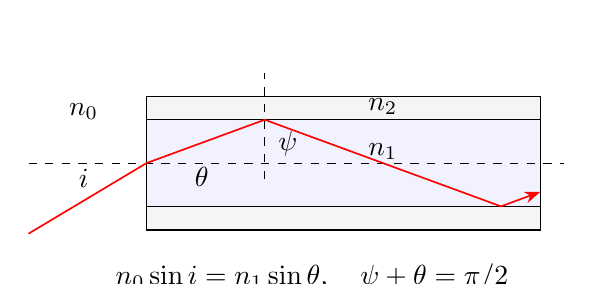
\begin{tikzpicture}[scale=1]
\draw[fill=gray!8] (0,-.85) rectangle(5,.85);
\draw[fill=blue!5] (0,-.55) rectangle(5,.55);
\draw[dashed] (-1.5,0)--(5.3,0);
\draw[arr,red] (-1.5,-.897)--(0,0)--(1.5,.55)--(4.5,-.55)--(5,-.3667);
\draw[dashed] (1.5,-.2)--(1.5,1.15);
\node at (-.8,-.2) {$i$};
\node at (.7,-.18) {$\theta$};
\node[right] at (1.55,.25) {$\psi$};
\node at (3,.15) {$n_1$}; \node at (3,.72) {$n_2$};
\node at (-.8,.65) {$n_0$};
\node at (2.1,-1.45) {$n_0\sin i=n_1\sin\theta,\quad\psi+\theta=\pi/2$};
\end{tikzpicture}
}
\ifdim\wd\diagrambox>.88\linewidth
\sbox{\diagrambox}{\resizebox{.88\linewidth}{!}{\usebox{\diagrambox}}}\fi
\ifdim\ht\diagrambox>.20\textheight
\resizebox{!}{.20\textheight}{\usebox{\diagrambox}}
\else\usebox{\diagrambox}\fi
\par\smallskip{\small 图6b　端面折射与芯包层全反射\par}\endgroup\end{minipage}\end{center}

（2）将光纤密绕\(N\)圈，首尾接于\(A\)，整个环路逆时针以\(\Omega\)转动。芯介质折射率为\(n_1\)，两束光真空波长为\(\lambda_0\)。求两束光传播\(N\)圈返回\(A\)的时间\(t_{\rm CCW},t_{\rm CW}\)、相位差，以及相位差与\(n_1\)的关系。

（3）旋转环形谐振腔半径为\(R\)，介质折射率\(n\)，\(R\Omega\ll c\)，腔和介质共同逆时针旋转。静止时模式满足\(2\pi R=m\lambda_{m0}\)，\(m\)为正整数、\(\lambda_{m0}\)为介质内波长。旋转时同一级次的CW、CCW共振模式有频率差\(\Delta f\)，求\(\Omega\)与\(\Delta f\)的关系。

\clearpage

\section{第 7
题　双黑洞旋近的辐射与轨道演化（40分）}\label{ux7b2c-7-ux9898-ux53ccux9ed1ux6d1eux65cbux8fd1ux7684ux8f90ux5c04ux4e0eux8f68ux9053ux6f14ux531640ux5206}

双黑洞并合分为旋近、并合、衰荡三个阶段。旋近阶段，两黑洞绕系统质心在同一平面内作近似圆周运动，机械能损失转为引力波辐射能，间距\(L\)逐渐减小。

在旋近阶段忽略黑洞自转与大小，将它们视为质量\(M,m\)的质点。系统除引力波辐射外没有能量耗散；不考虑辐射反作用的详细形式，轨道关系用牛顿引力近似。

\begin{center}
\begin{minipage}{\linewidth}
\centering\begingroup\sbox{\diagrambox}{\small
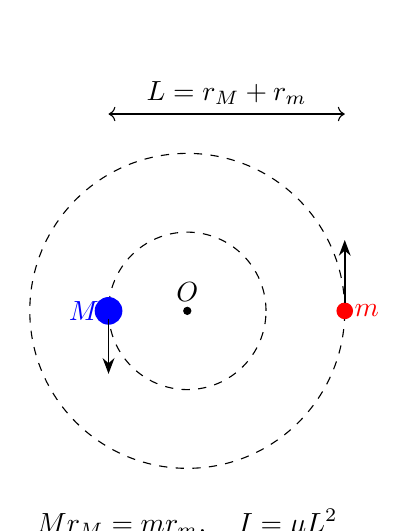
\begin{tikzpicture}[scale=1]
\draw[dashed] (0,0) circle(1); \draw[dashed] (0,0) circle(2);
\fill[blue] (-1,0) circle(5pt) node[left] {$M$};
\fill[red] (2,0) circle(3pt) node[right] {$m$};
\fill (0,0) circle(1.5pt) node[above] {$O$};
\draw[arr] (-1,-.1)--(-1,-.8); \draw[arr] (2,.1)--(2,.9);
\draw[<->] (-1,2.5)--(2,2.5) node[midway,above] {$L=r_M+r_m$};
\node at (0,-2.7) {$Mr_M=mr_m,\quad I=\mu L^2$};
\end{tikzpicture}
}
\ifdim\wd\diagrambox>.88\linewidth
\sbox{\diagrambox}{\resizebox{.88\linewidth}{!}{\usebox{\diagrambox}}}\fi
\ifdim\ht\diagrambox>.20\textheight
\resizebox{!}{.20\textheight}{\usebox{\diagrambox}}
\else\usebox{\diagrambox}\fi
\par\smallskip{\small 图7a　双质点绕共同质心旋近\par}\endgroup\end{minipage}\end{center}

（1）辐射功率与\(G\)正比，可与\(M,m,L\)、绕质心的转动惯量\(I\)、角速度\(\omega\)、辐射传播速度\(c\)有关。取描述转动体系的三个物理量，与\(G\)一起用量纲分析求功率形式，无量纲比例系数记为\(\alpha\)。

（2）已知\(t=0\)时两黑洞间距\(L_0\)，\(\alpha\)为已知常量。求两黑洞从\(t=0\)开始绕系统质心旋转360°所需时间。

（3）求当间距缩为\(L_0/2\)时，自初始时刻起旋转的度数。

\clearpage

\section{第 8
题　电光调制与并联谐振驱动（40分）}\label{ux7b2c-8-ux9898-ux7535ux5149ux8c03ux5236ux4e0eux5e76ux8054ux8c10ux632fux9a71ux52a840ux5206}

电光调制将电信号转入光信号。以铌酸锂晶体为例，折射率随外电场变化，使光程改变。起偏器\(P_1\)与检偏器\(P_2\)相互正交，透光轴分别沿\(x_1,x_2\)。长度\(l\)、厚度\(d\)的晶体位于二者之间，电场沿光的传播方向\(x_3\)，大小\(E\)，晶体两端面加电压\(V\)。

\begin{center}
\begin{minipage}{\linewidth}
\centering\begingroup\sbox{\diagrambox}{\small
\begin{tikzpicture}[scale=.85]
\draw[arr,thick] (-1,0)--(9,0) node[right] {$x_3$光};
\draw[very thick] (0,-.8)--(0,.8);
\node[above] at (0,.85) {$P_1\parallel x_1$};
\draw[fill=blue!5,thick] (1,-.6) rectangle(5,.6);
\node at (3,.2) {电光晶体};
\node at (1,-.85) {$+$};\node at (5,-.85) {$-$};
\draw[<->] (1,1.3)--(5,1.3) node[midway,above] {$l$};
\draw[<->] (1,-1.3)--(5,-1.3) node[midway,below] {$V,\ E=V/l$};
\draw[very thick] (6,-.8)--(6,.8); \node[above] at (6,.85) {$1/4$波片};
\draw[very thick] (7.6,-.8)--(7.6,.8); \node[above] at (7.8,1.4) {$P_2\parallel x_2$};
\draw[arr] (3,-3.8)--(3,-2.8) node[above] {$x_1$};
\draw[arr] (3,-3.8)--(4,-3.8) node[right] {$x_2$};
\draw[arr,blue] (3,-3.8)--(2.3,-3.1) node[left] {$x'_1$};
\draw[arr,red] (3,-3.8)--(3.7,-3.1) node[right] {$x'_2$};
\end{tikzpicture}
}
\ifdim\wd\diagrambox>.88\linewidth
\sbox{\diagrambox}{\resizebox{.88\linewidth}{!}{\usebox{\diagrambox}}}\fi
\ifdim\ht\diagrambox>.20\textheight
\resizebox{!}{.20\textheight}{\usebox{\diagrambox}}
\else\usebox{\diagrambox}\fi
\par\smallskip{\small 图8a　偏振分解、晶体与四分之一波片\par}\endgroup\end{minipage}\end{center}

真空波长\(\lambda_0\)的光经\(P_1\)后沿\(x_3\)入射，分解为晶体快轴\(x'_1\)与慢轴\(x'_2\)上的正交分量。两主轴与\(x_1,x_2\)均呈45°，折射率为

\[
n_{x'_1}=n_0-\frac12n_0^3\gamma E,\qquad
n_{x'_2}=n_0+\frac12n_0^3\gamma E.
\]

\(\gamma\)为材料常量。光出晶体后经过1/4波片，再由\(P_2\)检出。采用题图主轴对齐、波片给慢快分量额外\(+\pi/2\)延迟的约定。

（1）入射到晶体左端面的两分量电场为\(E_{x'_1}=E_0\cos\omega t\)、\(E_{x'_2}=E_0\cos\omega t\)。求经过晶体的相位变化和光强变化；出射两分量相位差为\(\pi\)时称晶体为1/2波片，求半波电压\(V_\pi\)。

（2）调制电压\(V=V_m\sin\omega_mt\)，\(V_m\ll V_\pi\)。先求不经过1/4波片、直接经\(P_2\)后的光强透过率与\(V\)的关系；再求经过1/4波片与\(P_2\)的透过率，指出1/4波片的作用。

（3）晶体的等效电路为并联电阻\(R\)和电容\(C\)，电源串联电阻\(R_m\)，\(R\gg R_m\)。开关断开时，证明当\(\omega_m\gg(R_mC)^{-1}\)，晶体实际电压\(|V_c|\ll|V|\)。

\begin{center}
\begin{minipage}{\linewidth}
\centering\begingroup\sbox{\diagrambox}{\small
\begin{tikzpicture}[scale=.9]
\draw[thick] (0,0)--(0,.6); \draw[thick] (0,1) circle(.4); \node at (0,1) {$V$};
\draw[thick] (0,1.4)--(0,2)--(.8,2);
\draw[thick] (.8,1.8) rectangle(1.8,2.2); \node[above] at (1.3,2.3) {$R_m$};
\draw[thick] (1.8,2)--(5.1,2);
\draw[thick] (3,2)--(3,1.4); \draw[thick] (2.8,.6) rectangle(3.2,1.4);
\node[left] at (2.8,1) {$R$};\draw[thick] (3,.6)--(3,0);
\draw[thick] (4.4,2)--(4.4,1.15); \draw[thick] (4.1,1.15)--(4.7,1.15);
\draw[thick] (4.1,.95)--(4.7,.95); \draw[thick] (4.4,.95)--(4.4,0);
\node[right] at (4.65,1) {$C$};
\draw (5.1,2) circle(1.5pt); \draw (5.8,2) circle(1.5pt);
\draw[thick] (5.1,2)--(5.7,2.35); \node at (5.4,2.7) {$S$};
\draw[thick] (5.8,2)--(7.7,2);
\draw[thick] (6.2,2)--(6.2,1.6);
\draw[thick,decorate,decoration={coil,aspect=.3,segment length=4pt,amplitude=3pt}] (6.2,1.6)--(6.2,.5);
\draw[thick] (6.2,.5)--(6.2,0); \node[right] at (6.5,1) {$L$};
\draw[thick] (7.7,2)--(7.7,1.4); \draw[thick] (7.5,.6) rectangle(7.9,1.4);
\node[right] at (7.9,1) {$R_L$}; \draw[thick] (7.7,.6)--(7.7,0)--(0,0);
\node at (4,-.8) {闭合$S$接入并联$L,R_L$};
\end{tikzpicture}
}
\ifdim\wd\diagrambox>.88\linewidth
\sbox{\diagrambox}{\resizebox{.88\linewidth}{!}{\usebox{\diagrambox}}}\fi
\ifdim\ht\diagrambox>.20\textheight
\resizebox{!}{.20\textheight}{\usebox{\diagrambox}}
\else\usebox{\diagrambox}\fi
\par\smallskip{\small 图8b　电源与晶体并联谐振补偿\par}\endgroup\end{minipage}\end{center}

（4）为提高调制效率，闭合开关，加入与晶体并联的谐振回路，电感为\(L\)、负载电阻为\(R_L\)。试证明\(|V_c|\simeq|V|\)。

\end{document}
